\documentclass{article}

\usepackage[margin=1in]{geometry}
\usepackage{amsmath}
\usepackage{graphicx}
\usepackage{multicol}
\usepackage{fancyvrb}
\usepackage{bibentry}
\usepackage[shortlabels]{enumitem}
\usepackage{tikz}

\newcommand{\fig}[3]{ 
	\begin{figure}[h]
		\centering
		\caption{#3}
		\includegraphics[width=#2\textwidth]{pics/#1}
		\label{fig:#1}
	\end{figure} 
}

\begin{document}
\title{ESOF 422 - Homework 5}
\author{Nathan Stouffer \and Kevin Browder}

\maketitle
\newpage
\section*{Question 1}
How else could we compare test criteria besides subsumption?

\newpage
\section*{Question 2}
\subsection*{Book Question 4}
We consider the following graph
\begin{flalign*}
\indent & N = \{ 1, 2, 3, 4 \} & \\
		& N_0 = \{ 1 \} \\
		& N_f = \{ 4 \} \\
		& E = \{ (1, 2), (2, 3), (3, 2), (2, 4) \}
\end{flalign*}
\begin{enumerate}[(a)]
	\item We depict the graph below
		\begin{center}
			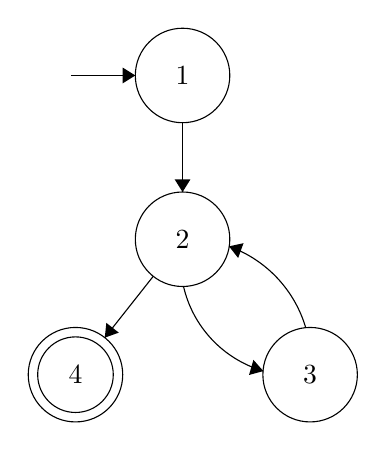
\begin{tikzpicture}[scale=0.2]
				\tikzstyle{every node}+=[inner sep=0pt]
				\draw [black] (23.4,-7.3) circle (3);
				\draw (23.4,-7.3) node {$1$};
				\draw [black] (23.4,-17.7) circle (3);
				\draw (23.4,-17.7) node {$2$};
				\draw [black] (31.5,-26.3) circle (3);
				\draw (31.5,-26.3) node {$3$};
				\draw [black] (16.6,-26.3) circle (3);
				\draw (16.6,-26.3) node {$4$};
				\draw [black] (16.6,-26.3) circle (2.4);
				\draw [black] (16.3,-7.3) -- (20.4,-7.3);
				\fill [black] (20.4,-7.3) -- (19.6,-6.8) -- (19.6,-7.8);
				\draw [black] (23.4,-10.3) -- (23.4,-14.7);
				\fill [black] (23.4,-14.7) -- (23.9,-13.9) -- (22.9,-13.9);
				\draw [black] (28.53,-26.065) arc (-106.28494:-167.14492:7.305);
				\fill [black] (28.53,-26.07) -- (27.9,-25.36) -- (27.62,-26.32);
				\draw [black] (26.347,-18.152) arc (70.30554:16.2646:7.83);
				\fill [black] (26.35,-18.15) -- (26.93,-18.89) -- (27.27,-17.95);
				\draw [black] (21.54,-20.05) -- (18.46,-23.95);
				\fill [black] (18.46,-23.95) -- (19.35,-23.63) -- (18.56,-23.01);
			\end{tikzpicture}
		\end{center}
	\item There are no test paths that achieve Node Coverage but not Edge Coverage. For the above graph, any path that satisfies Node Coverage must also satisfy Edge Coverage. This is because the graph has no branches to follow (only a cycle). For example, the test path [1, 2, 3, 2, 4] satisfies NC and EC.
	\item A test path that satisfies EC but not EPC is [1, 2, 3, 2, 4]. This does not achieve EPC because it is missing [3, 2, 3]
	\item The set of test paths that satisfy EPC is $\{  [1, 2, 3, 2, 3, 2, 4], [1, 2, 4 ] \}$
\end{enumerate}

\subsection*{Book Question 5}
We now consider the following graph
\begin{flalign*}
	\indent & N = \{ 1, 2, 3, 4, 5, 6, 7 \} & \\
			& N_0 = \{ 1 \} \\
			& N_f = \{ 7 \} \\
			& E = \{ (1,2), (1, 7), (2, 3), (2, 4), (3, 2), (4, 5), (4, 6), (5, 6), (6, 1) \}
\end{flalign*}
We also consider the following (candidate) test paths
\begin{flalign*}
\indent & p_1 = [ 1, 2, 4, 5, 6, 1, 7 ] & \\
		& p_2 = [ 1, 2, 3, 2, 4, 6, 1, 7 ] \\
		& p_3 = [ 1, 2, 3, 2, 4, 5, 6, 1, 7 ]
\end{flalign*}
\begin{enumerate}[(a)]
	\item We depict the graph below
		\begin{center}
			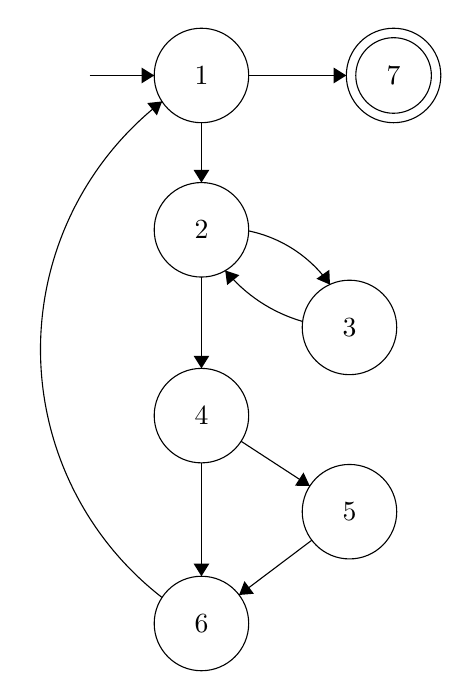
\begin{tikzpicture}[scale=0.2]
			\tikzstyle{every node}+=[inner sep=0pt]
			\draw [black] (21.9,-7.5) circle (3);
			\draw (21.9,-7.5) node {$1$};
			\draw [black] (21.9,-17.3) circle (3);
			\draw (21.9,-17.3) node {$2$};
			\draw [black] (31.3,-23.5) circle (3);
			\draw (31.3,-23.5) node {$3$};
			\draw [black] (21.9,-29.1) circle (3);
			\draw (21.9,-29.1) node {$4$};
			\draw [black] (31.3,-35.2) circle (3);
			\draw (31.3,-35.2) node {$5$};
			\draw [black] (21.9,-42.3) circle (3);
			\draw (21.9,-42.3) node {$6$};
			\draw [black] (34.1,-7.5) circle (3);
			\draw (34.1,-7.5) node {$7$};
			\draw [black] (34.1,-7.5) circle (2.4);
			\draw [black] (14.8,-7.5) -- (18.9,-7.5);
			\fill [black] (18.9,-7.5) -- (18.1,-7) -- (18.1,-8);
			\draw [black] (24.9,-7.5) -- (31.1,-7.5);
			\fill [black] (31.1,-7.5) -- (30.3,-7) -- (30.3,-8);
			\draw [black] (21.9,-10.5) -- (21.9,-14.3);
			\fill [black] (21.9,-14.3) -- (22.4,-13.5) -- (21.4,-13.5);
			\draw [black] (24.883,-17.367) arc (78.41457:34.76978:8.348);
			\fill [black] (30.06,-20.78) -- (30.02,-19.84) -- (29.2,-20.41);
			\draw [black] (21.9,-20.3) -- (21.9,-26.1);
			\fill [black] (21.9,-26.1) -- (22.4,-25.3) -- (21.4,-25.3);
			\draw [black] (28.335,-23.123) arc (-105.973:-140.84265:9.84);
			\fill [black] (23.41,-19.88) -- (23.53,-20.81) -- (24.31,-20.18);
			\draw [black] (24.42,-30.73) -- (28.78,-33.57);
			\fill [black] (28.78,-33.57) -- (28.38,-32.71) -- (27.84,-33.55);
			\draw [black] (21.9,-32.1) -- (21.9,-39.3);
			\fill [black] (21.9,-39.3) -- (22.4,-38.5) -- (21.4,-38.5);
			\draw [black] (19.399,-40.648) arc (-127.76682:-232.23318:19.921);
			\fill [black] (19.4,-9.15) -- (18.46,-9.25) -- (19.07,-10.04);
			\draw [black] (28.91,-37.01) -- (24.29,-40.49);
			\fill [black] (24.29,-40.49) -- (25.23,-40.41) -- (24.63,-39.61);
			\end{tikzpicture}
		\end{center}
	\item We now list the test requirements for EPC on the above graph. TR = \{ [1, 2, 3], [1, 2, 4], [2, 3, 2], [2, 4, 5], [2, 4, 6], [3, 2, 3], [3, 2, 4], [4, 5, 6], [4, 6, 1], [5, 6, 1], [6, 1, 2], [6, 1, 7] \}
	\item The given set of test paths ($p_1$, $p_2$, $p_3$) do not satisfy Edge-Pair Coverage. They are missing [3, 2, 3] and [6, 2, 1] so they do not satisfy EPC.
	\item This question considers the simple path [3, 2, 4, 5, 6] and the test path [1, 2, 3, 2, 4, 6, 1, 2, 4, 5, 6, 1, 7]. For the given paths, the test path does not tour the simple path directly. It takes a side trip through the path [6, 1, 2].
	\item We now give the test requirements for Node Coverage, Edge Coverage, and Prime Path Coverage. \\\\	
	$TR_{NC} =$ \{ [1], [2], [3], [4], [5], [6], [7] \} \\\\
	$ TR_{EC} =$ \{ [1, 2], [1, 7], [2, 3], [2, 4], [3, 2], [4, 5], [4, 6], [5, 6], [6, 1] \} \\\\
	$TR_{PPC} =$ \{ [3, 2, 4, 5, 6, 1, 7], 
					[1, 2, 4, 5, 6 ,1], 
					[2, 4, 5, 6, 1, 2], 
					[3, 2, 4, 6, 1, 7],
					[4, 5, 6, 1, 2, 3], 
					[4, 5, 6, 1, 2, 4], 
					[5, 6, 1, 2, 4, 5], 
					[6, 1, 2, 4, 5, 6], 
					[6, 1, 2, 4, 6], 
					[1, 2, 4, 6, 1], 
					[2, 4, 6, 1, 2],
					[4, 6, 1, 2, 3], 
					[4, 6, 1, 2, 4], 
					[2, 3, 2], 
					[3, 2, 3] \}

	\item From $ \{ p_1, p_2, p_3 \}$, the test path $p_3 = [1, 2, 3, 2, 4, 5, 6, 1, 7]$ satisfies Node Coverage but not Edge Coverage.
	\item From $ \{ p_1, p_2, p_3 \}$, the test paths 
	$p_1 = [1, 2, 4, 5, 6, 1, 7]$ and  $p_2 = [1, 2, 3, 2, 4, 6, 1, 7]$ achieve Edge Coverage but not Prime Path Coverage.
\end{enumerate}

\newpage
\section*{Question 3}
Question 3 asks us to implement an algorithm that returns that prime paths of a graph. We do this with a Java implementation. Our program consists of two classes: Path and Graph. \\\\
The Path class is essentially just a list of nodes in the path. Operations that can be called on a path are queries that tell whether a given path visits a node, tours a subpath, or is a simple path. \\\\
The Graph class 

\end{document}